% Options for packages loaded elsewhere
\PassOptionsToPackage{unicode}{hyperref}
\PassOptionsToPackage{hyphens}{url}
%
\documentclass[
  ignorenonframetext,
]{beamer}
\usepackage{pgfpages}
\setbeamertemplate{caption}[numbered]
\setbeamertemplate{caption label separator}{: }
\setbeamercolor{caption name}{fg=normal text.fg}
\beamertemplatenavigationsymbolsempty
% Prevent slide breaks in the middle of a paragraph
\widowpenalties 1 10000
\raggedbottom
\setbeamertemplate{part page}{
  \centering
  \begin{beamercolorbox}[sep=16pt,center]{part title}
    \usebeamerfont{part title}\insertpart\par
  \end{beamercolorbox}
}
\setbeamertemplate{section page}{
  \centering
  \begin{beamercolorbox}[sep=12pt,center]{section title}
    \usebeamerfont{section title}\insertsection\par
  \end{beamercolorbox}
}
\setbeamertemplate{subsection page}{
  \centering
  \begin{beamercolorbox}[sep=8pt,center]{subsection title}
    \usebeamerfont{subsection title}\insertsubsection\par
  \end{beamercolorbox}
}
\AtBeginPart{
  \frame{\partpage}
}
\AtBeginSection{
  \ifbibliography
  \else
    \frame{\sectionpage}
  \fi
}
\AtBeginSubsection{
  \frame{\subsectionpage}
}

\usepackage{amsmath,amssymb}
\usepackage{iftex}
\ifPDFTeX
  \usepackage[T1]{fontenc}
  \usepackage[utf8]{inputenc}
  \usepackage{textcomp} % provide euro and other symbols
\else % if luatex or xetex
  \usepackage{unicode-math}
  \defaultfontfeatures{Scale=MatchLowercase}
  \defaultfontfeatures[\rmfamily]{Ligatures=TeX,Scale=1}
\fi
\usepackage{lmodern}
\ifPDFTeX\else  
    % xetex/luatex font selection
\fi
% Use upquote if available, for straight quotes in verbatim environments
\IfFileExists{upquote.sty}{\usepackage{upquote}}{}
\IfFileExists{microtype.sty}{% use microtype if available
  \usepackage[]{microtype}
  \UseMicrotypeSet[protrusion]{basicmath} % disable protrusion for tt fonts
}{}
\makeatletter
\@ifundefined{KOMAClassName}{% if non-KOMA class
  \IfFileExists{parskip.sty}{%
    \usepackage{parskip}
  }{% else
    \setlength{\parindent}{0pt}
    \setlength{\parskip}{6pt plus 2pt minus 1pt}}
}{% if KOMA class
  \KOMAoptions{parskip=half}}
\makeatother
\usepackage{xcolor}
\newif\ifbibliography
\setlength{\emergencystretch}{3em} % prevent overfull lines
\setcounter{secnumdepth}{-\maxdimen} % remove section numbering


\providecommand{\tightlist}{%
  \setlength{\itemsep}{0pt}\setlength{\parskip}{0pt}}\usepackage{longtable,booktabs,array}
\usepackage{calc} % for calculating minipage widths
\usepackage{caption}
% Make caption package work with longtable
\makeatletter
\def\fnum@table{\tablename~\thetable}
\makeatother
\usepackage{graphicx}
\makeatletter
\newsavebox\pandoc@box
\newcommand*\pandocbounded[1]{% scales image to fit in text height/width
  \sbox\pandoc@box{#1}%
  \Gscale@div\@tempa{\textheight}{\dimexpr\ht\pandoc@box+\dp\pandoc@box\relax}%
  \Gscale@div\@tempb{\linewidth}{\wd\pandoc@box}%
  \ifdim\@tempb\p@<\@tempa\p@\let\@tempa\@tempb\fi% select the smaller of both
  \ifdim\@tempa\p@<\p@\scalebox{\@tempa}{\usebox\pandoc@box}%
  \else\usebox{\pandoc@box}%
  \fi%
}
% Set default figure placement to htbp
\def\fps@figure{htbp}
\makeatother

\makeatletter
\@ifpackageloaded{caption}{}{\usepackage{caption}}
\AtBeginDocument{%
\ifdefined\contentsname
  \renewcommand*\contentsname{Table of contents}
\else
  \newcommand\contentsname{Table of contents}
\fi
\ifdefined\listfigurename
  \renewcommand*\listfigurename{List of Figures}
\else
  \newcommand\listfigurename{List of Figures}
\fi
\ifdefined\listtablename
  \renewcommand*\listtablename{List of Tables}
\else
  \newcommand\listtablename{List of Tables}
\fi
\ifdefined\figurename
  \renewcommand*\figurename{Figure}
\else
  \newcommand\figurename{Figure}
\fi
\ifdefined\tablename
  \renewcommand*\tablename{Table}
\else
  \newcommand\tablename{Table}
\fi
}
\@ifpackageloaded{float}{}{\usepackage{float}}
\floatstyle{ruled}
\@ifundefined{c@chapter}{\newfloat{codelisting}{h}{lop}}{\newfloat{codelisting}{h}{lop}[chapter]}
\floatname{codelisting}{Listing}
\newcommand*\listoflistings{\listof{codelisting}{List of Listings}}
\makeatother
\makeatletter
\makeatother
\makeatletter
\@ifpackageloaded{caption}{}{\usepackage{caption}}
\@ifpackageloaded{subcaption}{}{\usepackage{subcaption}}
\makeatother

\usepackage{bookmark}

\IfFileExists{xurl.sty}{\usepackage{xurl}}{} % add URL line breaks if available
\urlstyle{same} % disable monospaced font for URLs
\hypersetup{
  pdftitle={\ldots to Large Language Models},
  pdfauthor={Pablo Winant},
  hidelinks,
  pdfcreator={LaTeX via pandoc}}


\title{\ldots to Large Language Models}
\subtitle{AI for Research, ESCP, 2024-2025}
\author{Pablo Winant}
\date{2024-11-29}

\begin{document}
\frame{\titlepage}


\section{What does GPT do? Text
completion.}\label{what-does-gpt-do-text-completion.}

\begin{frame}[fragile]{Do you like poetry?}
\phantomsection\label{do-you-like-poetry}
\pause

\begin{quote}
A rose is a rose is {a rose}
\end{quote}

\pause

\begin{verbatim}
Gertrude Stein
\end{verbatim}

\pause

\begin{quote}
Brexit means Brexit means {Brexit}
\end{quote}

\pause

\begin{verbatim}
John Crace
\end{verbatim}

\pause

\begin{quote}
Elementary my dear {Watson}
\end{quote}

\pause

\begin{verbatim}
P.G. Woodehouse
\end{verbatim}

\pause
\end{frame}

\begin{frame}{}
\phantomsection\label{section}
\begin{quote}
There is an easy way for the government to end the strike without
withdrawing the pension reform,
\end{quote}

\pause
\end{frame}

\begin{frame}{Complete Text}
\phantomsection\label{complete-text}
Generative language models perform \emph{text completion}

They generate plausible\footnote<.->{here, plausible, means that it is
  more likely to be a correct text written by a human, rather than
  otherwise} text following a prompt.

The type of answer, will depend on the kind of prompt.
\end{frame}

\begin{frame}[fragile]{GPT Playground}
\phantomsection\label{gpt-playground}
To use GPT-4 profficiently, you have to experiment with the prompt.

\begin{itemize}
\tightlist
\item
  try the \href{https://platform.openai.com/playground}{Playground mode}
\end{itemize}

It is the same as learning how to do google queries

\begin{itemize}
\tightlist
\item
  altavista: \texttt{+noir\ +film\ -"pinot\ noir"}
\item
  nowadays: ???
\end{itemize}

``Prompting'' is becoming a discipline in itself\ldots{} (or is it?)
\end{frame}

\begin{frame}{Some Examples}
\phantomsection\label{some-examples}
By providing enough \emph{context}, it is possible to perform amazing
tasks

\href{https://gpt4demo.com/}{Look at the demos}
\end{frame}

\section{What is a language model?}\label{what-is-a-language-model}

\begin{frame}{Language Models and Cryptography}
\phantomsection\label{language-models-and-cryptography}
\pandocbounded{\includegraphics[keepaspectratio]{assets/code-secret.webp}}

The Caesar code
\end{frame}

\begin{frame}{}
\phantomsection\label{section-1}
\begin{figure}[H]

{\centering \pandocbounded{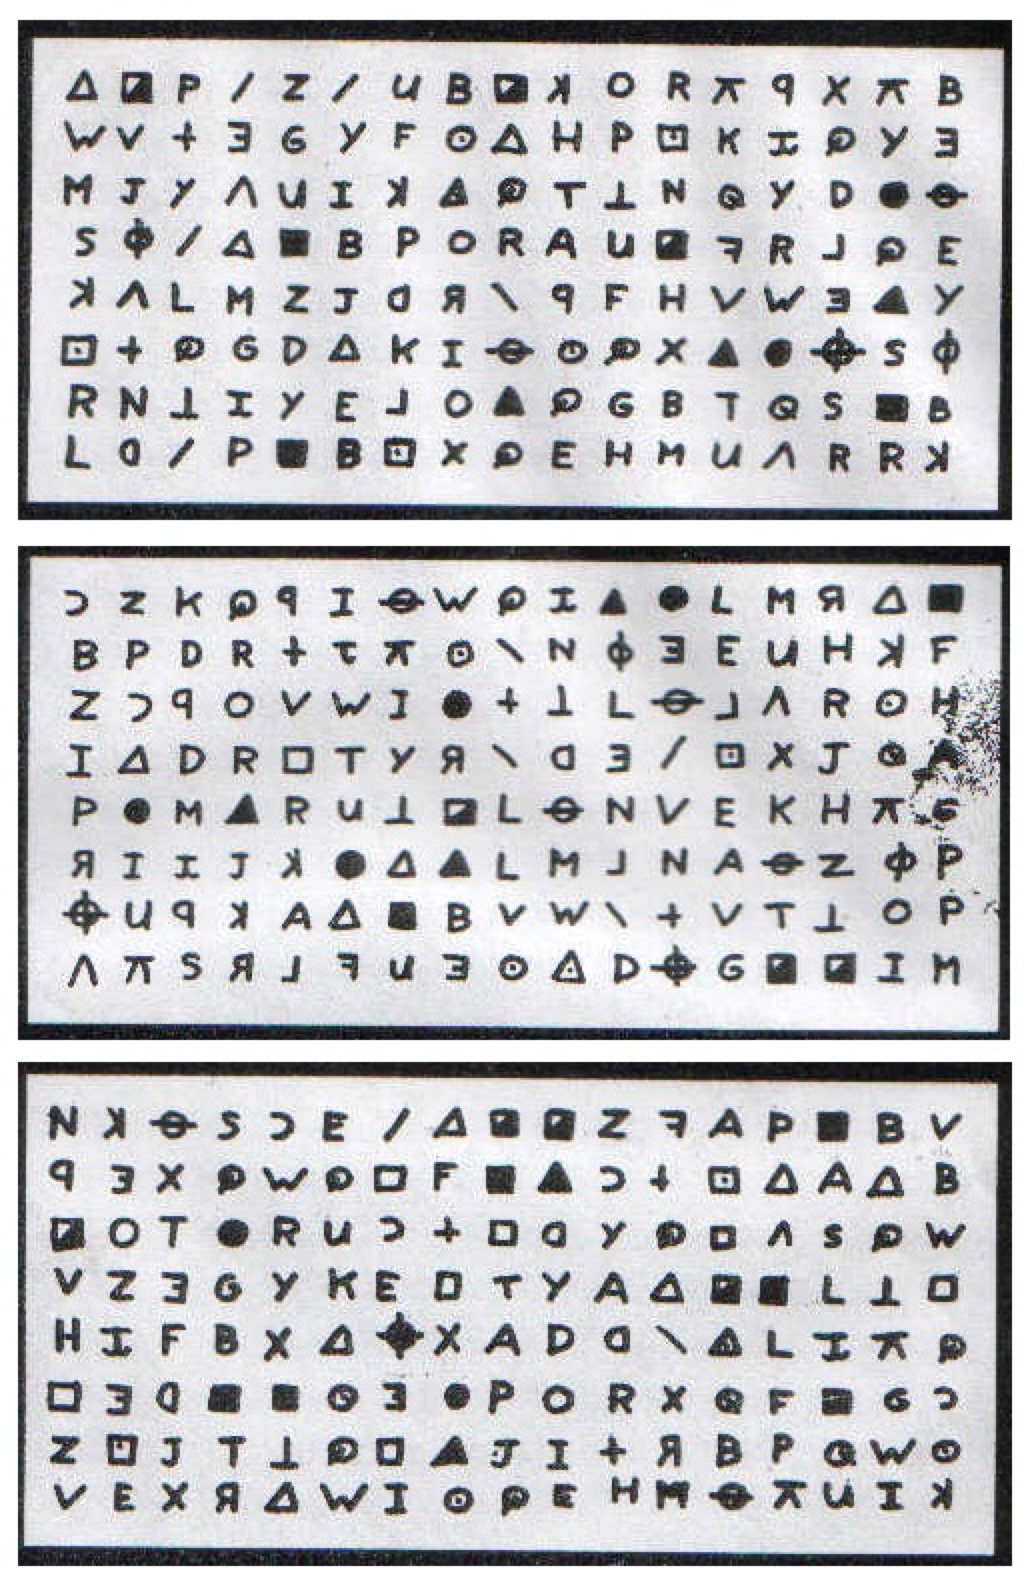
\includegraphics[keepaspectratio]{assets/zodiac_408.png}}

}

\caption{Zodiac 408 Cipher}

\end{figure}%
\end{frame}

\begin{frame}{}
\phantomsection\label{section-2}
\begin{figure}

\begin{minipage}{0.50\linewidth}

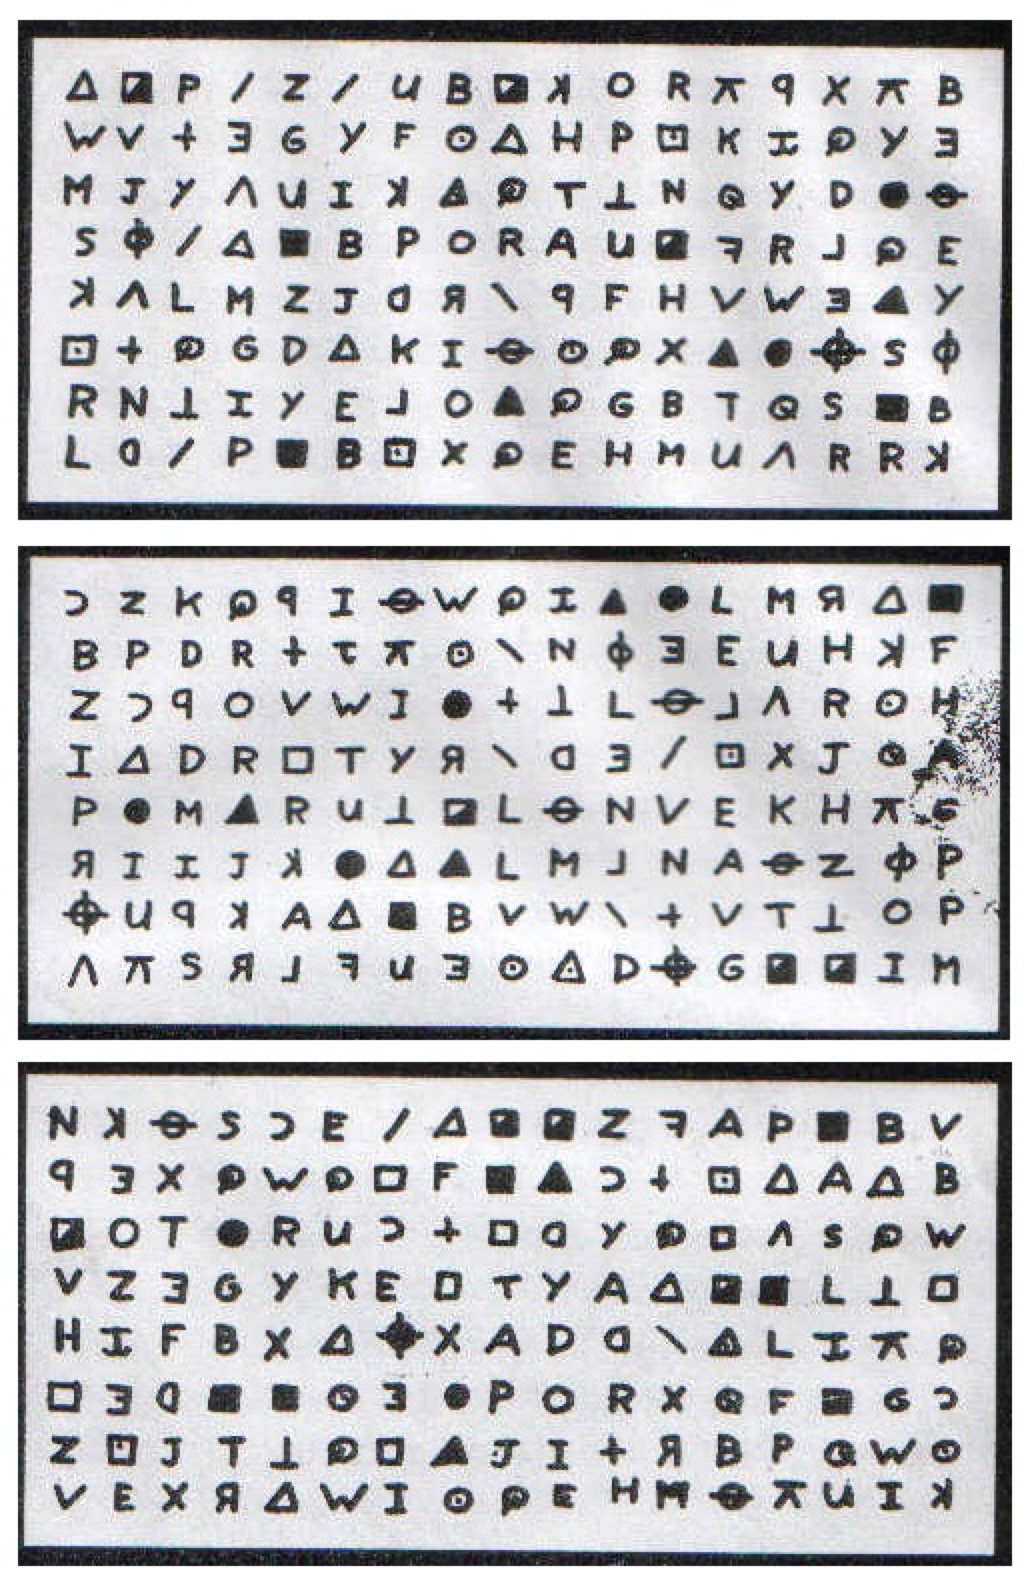
\includegraphics[width=0.2\linewidth,height=\textheight,keepaspectratio]{assets/zodiac_408.png}

\subcaption{\label{}Zodiac 408 Cipher}
\end{minipage}%
%
\begin{minipage}{0.50\linewidth}

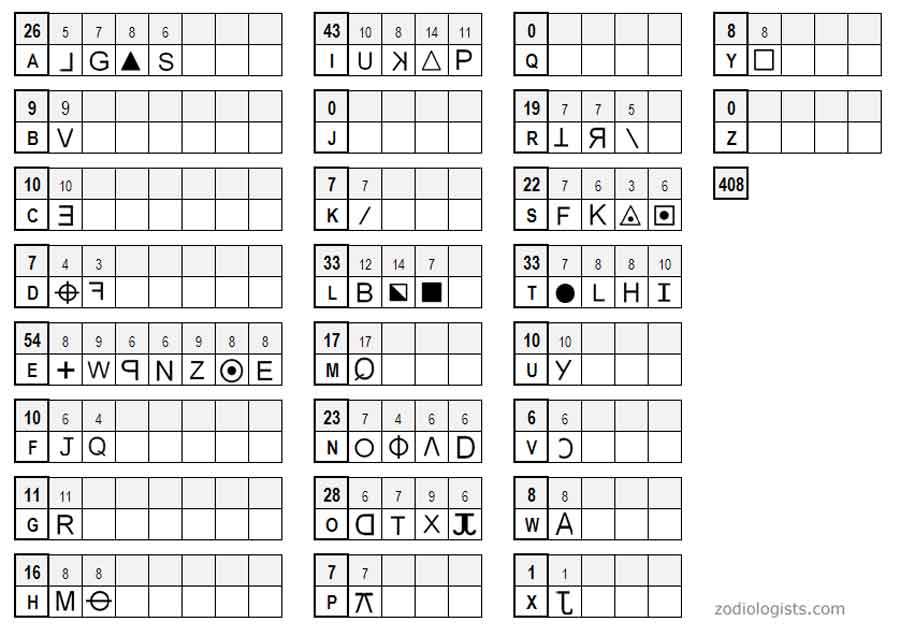
\includegraphics[width=0.4\linewidth,height=\textheight,keepaspectratio]{assets/408_solution.jpg}

\subcaption{\label{}Key for Zodiac 408}
\end{minipage}%

\caption{\label{fig-elephants}Solved in a week by Bettye and Donald
Harden using frequency tables.}

\end{figure}%
\end{frame}

\begin{frame}{}
\phantomsection\label{section-3}
Later in 2001, in a prison, somewhere in California

\pandocbounded{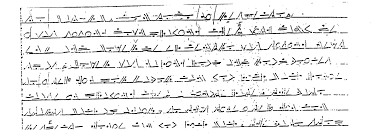
\includegraphics[keepaspectratio]{assets/prison.png}}

\pause

Solved by Stanford's
\href{https://math.uchicago.edu/~shmuel/Network-course-readings/MCMCRev.pdf}{Persi
Diaconis} and his students using Monte Carlo Markov Chains
\end{frame}

\begin{frame}{Monte Carlo Markov Chains}
\phantomsection\label{monte-carlo-markov-chains}
Take a letter \(x_n\), what is the probability of the next letter being
\(x_{n+1}\)?

\[\pi_{X,Y} = P(x_{n+1}=Y, x_{n}=X)\]

for \(X=\{a, b, .... , z\} , Y=\{a,b,c, ... z\}\)

The language model can be trained using dataset of english language.

And used to determine whether a given cipher-key is consistent with
english language.

It yields a very efficient algorithm to decode any caesar code (with
very small sample)
\end{frame}

\begin{frame}[fragile]{MCMC to generate text}
\phantomsection\label{mcmc-to-generate-text}
MCMCs can also be used to generate text:

\begin{itemize}
\tightlist
\item
  take initial prompt: \texttt{I\ think\ therefore\ I}

  \begin{itemize}
  \tightlist
  \item
    last letter is \texttt{I}
  \item
    most plausible character afterwards is \texttt{}
  \item
    most plausible character afterwards is \texttt{I}
  \end{itemize}
\item
  Result: \texttt{I\ think\ therefore\ I\ I\ I\ I\ I\ I}
\end{itemize}

Not good but promising (🤷)
\end{frame}

\begin{frame}[fragile]{MCMC to generate text}
\phantomsection\label{mcmc-to-generate-text-1}
Going further

\begin{itemize}
\tightlist
\item
  augment memory

  \begin{itemize}
  \tightlist
  \item
    \texttt{fore\ I}\textgreater{} ???
  \end{itemize}
\item
  change basic unit (use phonems or words)
\end{itemize}

An example using
\href{https://towardsdatascience.com/text-generation-with-markov-chains-an-introduction-to-using-markovify-742e6680dc33}{MCMC}

\begin{itemize}
\tightlist
\item
  using words and 3 states
  \texttt{He\ ha\ ‘s\ kill’d\ me\ Mother\ ,\ Run\ away\ I\ pray\ you\ Oh\ this\ is\ Counter\ you\ false\ Danish\ Dogges\ .}
\end{itemize}
\end{frame}

\begin{frame}[fragile]{Big MCMC}
\phantomsection\label{big-mcmc}
Can we augment memory?

\begin{itemize}
\tightlist
\item
  if you want to compute the most frequent letter (among \texttt{26})
  after \texttt{50} letters, you need to take into account
  \texttt{5.6061847e+70} combinations !

  \begin{itemize}
  \tightlist
  \item
    impossible to store, let alone do the training
  \end{itemize}
\item
  but some combinations are useless:

  \begin{itemize}
  \tightlist
  \item
    \texttt{wjai\ dfni}
  \item
    \texttt{Despite\ the\ constant\ negative\ press\ covfefe} {🤔}
  \end{itemize}
\end{itemize}
\end{frame}

\begin{frame}{Neural Networks}
\phantomsection\label{neural-networks}
\begin{columns}[T]
\begin{column}{0.48\linewidth}
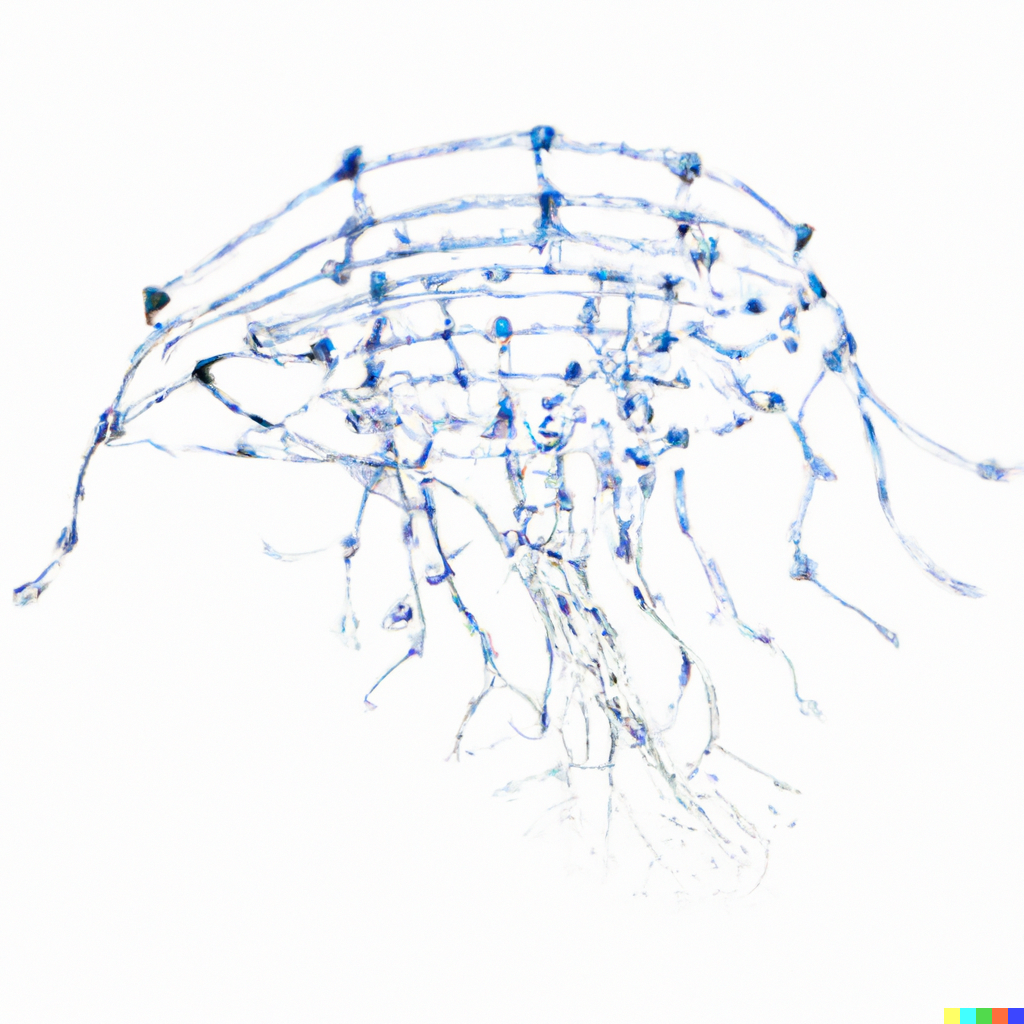
\includegraphics[width=0.6\linewidth,height=\textheight,keepaspectratio]{assets/glowing_nn.png}
\end{column}

\begin{column}{0.48\linewidth}
\begin{figure}[H]

{\centering 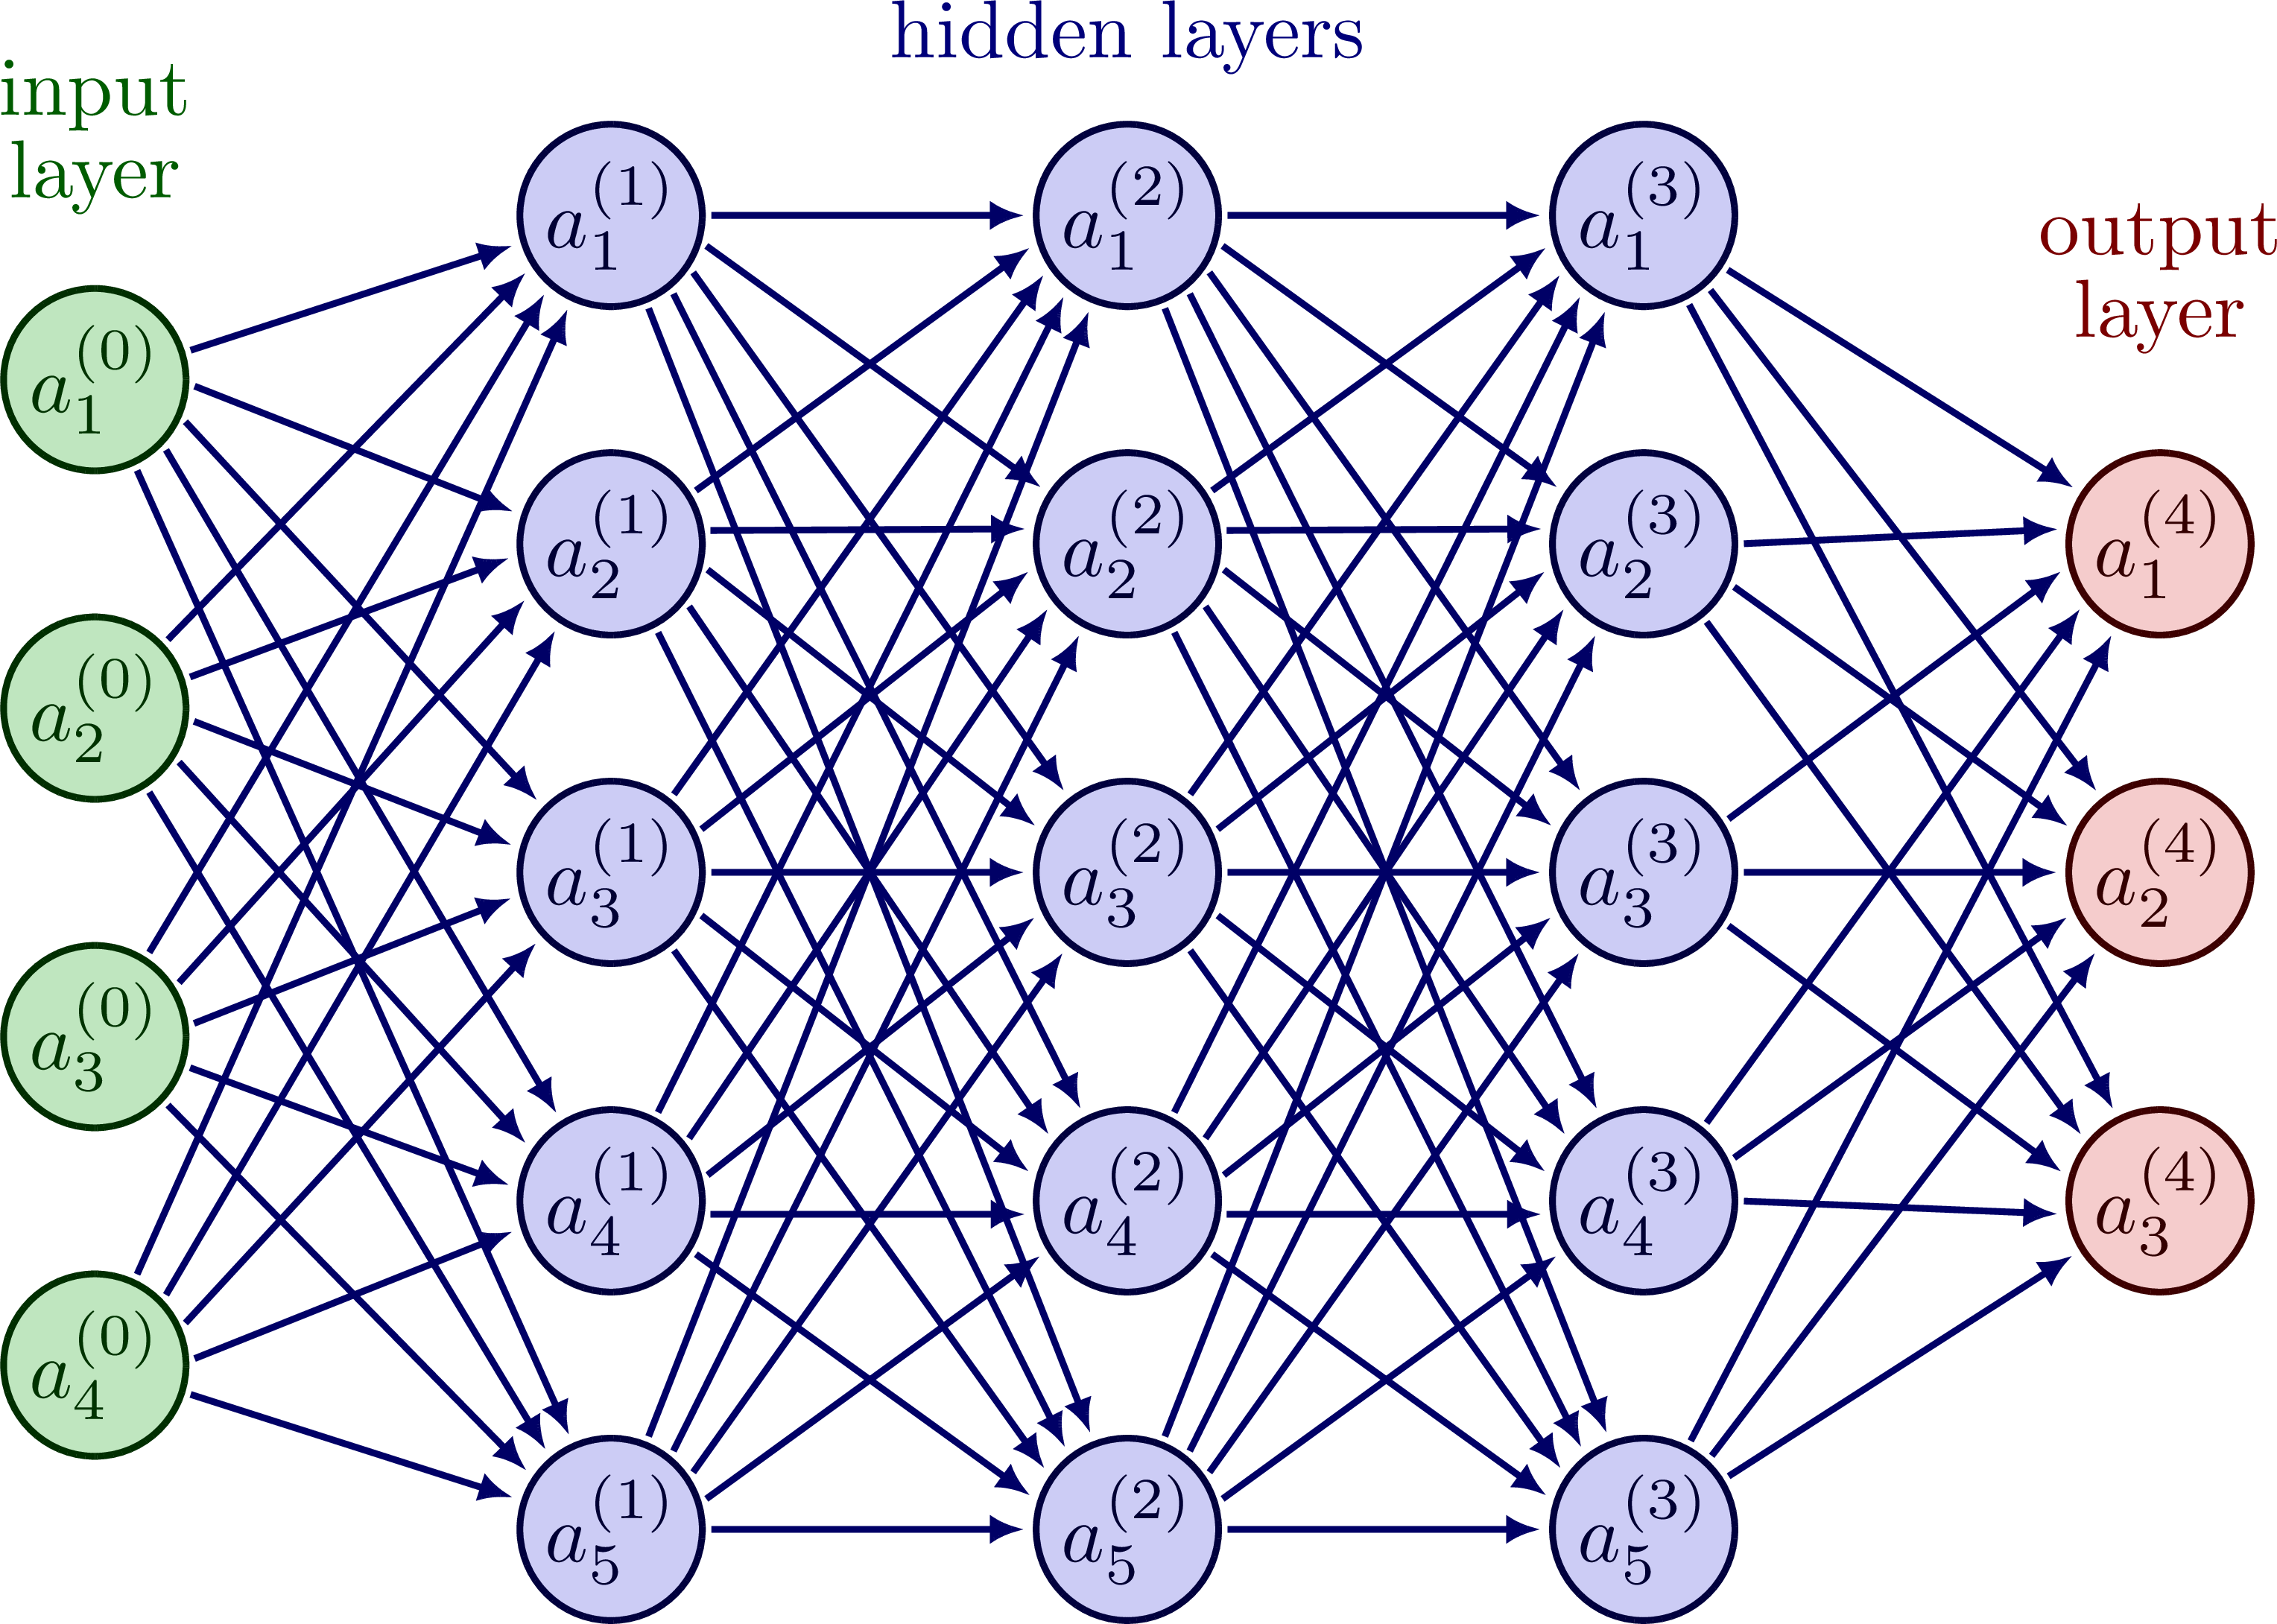
\includegraphics[width=0.6\linewidth,height=\textheight,keepaspectratio]{assets/neural_networks.png}

}

\caption{Neural Network}

\end{figure}%
\end{column}
\end{columns}

\begin{itemize}
\tightlist
\item
  Neural networks make it possible to increase the state-space to
  represent
\end{itemize}

\[\forall X, P(x_n=X| x_{n-1}, ..., x_{n-k}) = \varphi^{NL}( x_{n-1}, ..., x_{n-k}; \theta )\]

with a smaller vector of parameters \(\theta\)

\begin{itemize}
\tightlist
\item
  Neural netowrks reduce endogenously the dimensionality.
\end{itemize}
\end{frame}

\begin{frame}{Recurrent Neural Networks}
\phantomsection\label{recurrent-neural-networks}
\begin{columns}[T]
\begin{column}{0.48\linewidth}
In 2015
\end{column}

\begin{column}{0.48\linewidth}
\pandocbounded{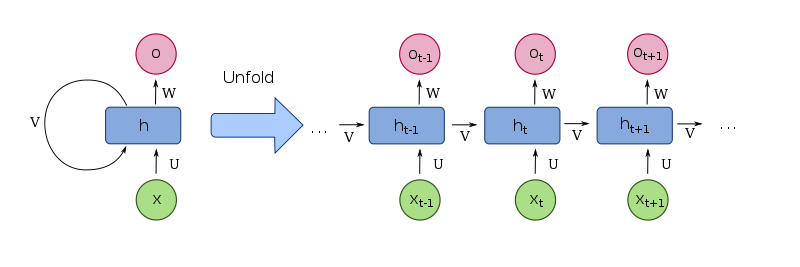
\includegraphics[keepaspectratio]{assets/Recurrent_neural_network_unfold.svg.png}}

\begin{itemize}
\tightlist
\item
  \textbf{Neural Network} reduce dimensionality of data discovering
  structure
\item
  hidden state encodes meaning of the model so far
\end{itemize}
\end{column}
\end{columns}
\end{frame}

\begin{frame}{Long Short Term Memory}
\phantomsection\label{long-short-term-memory}
\pandocbounded{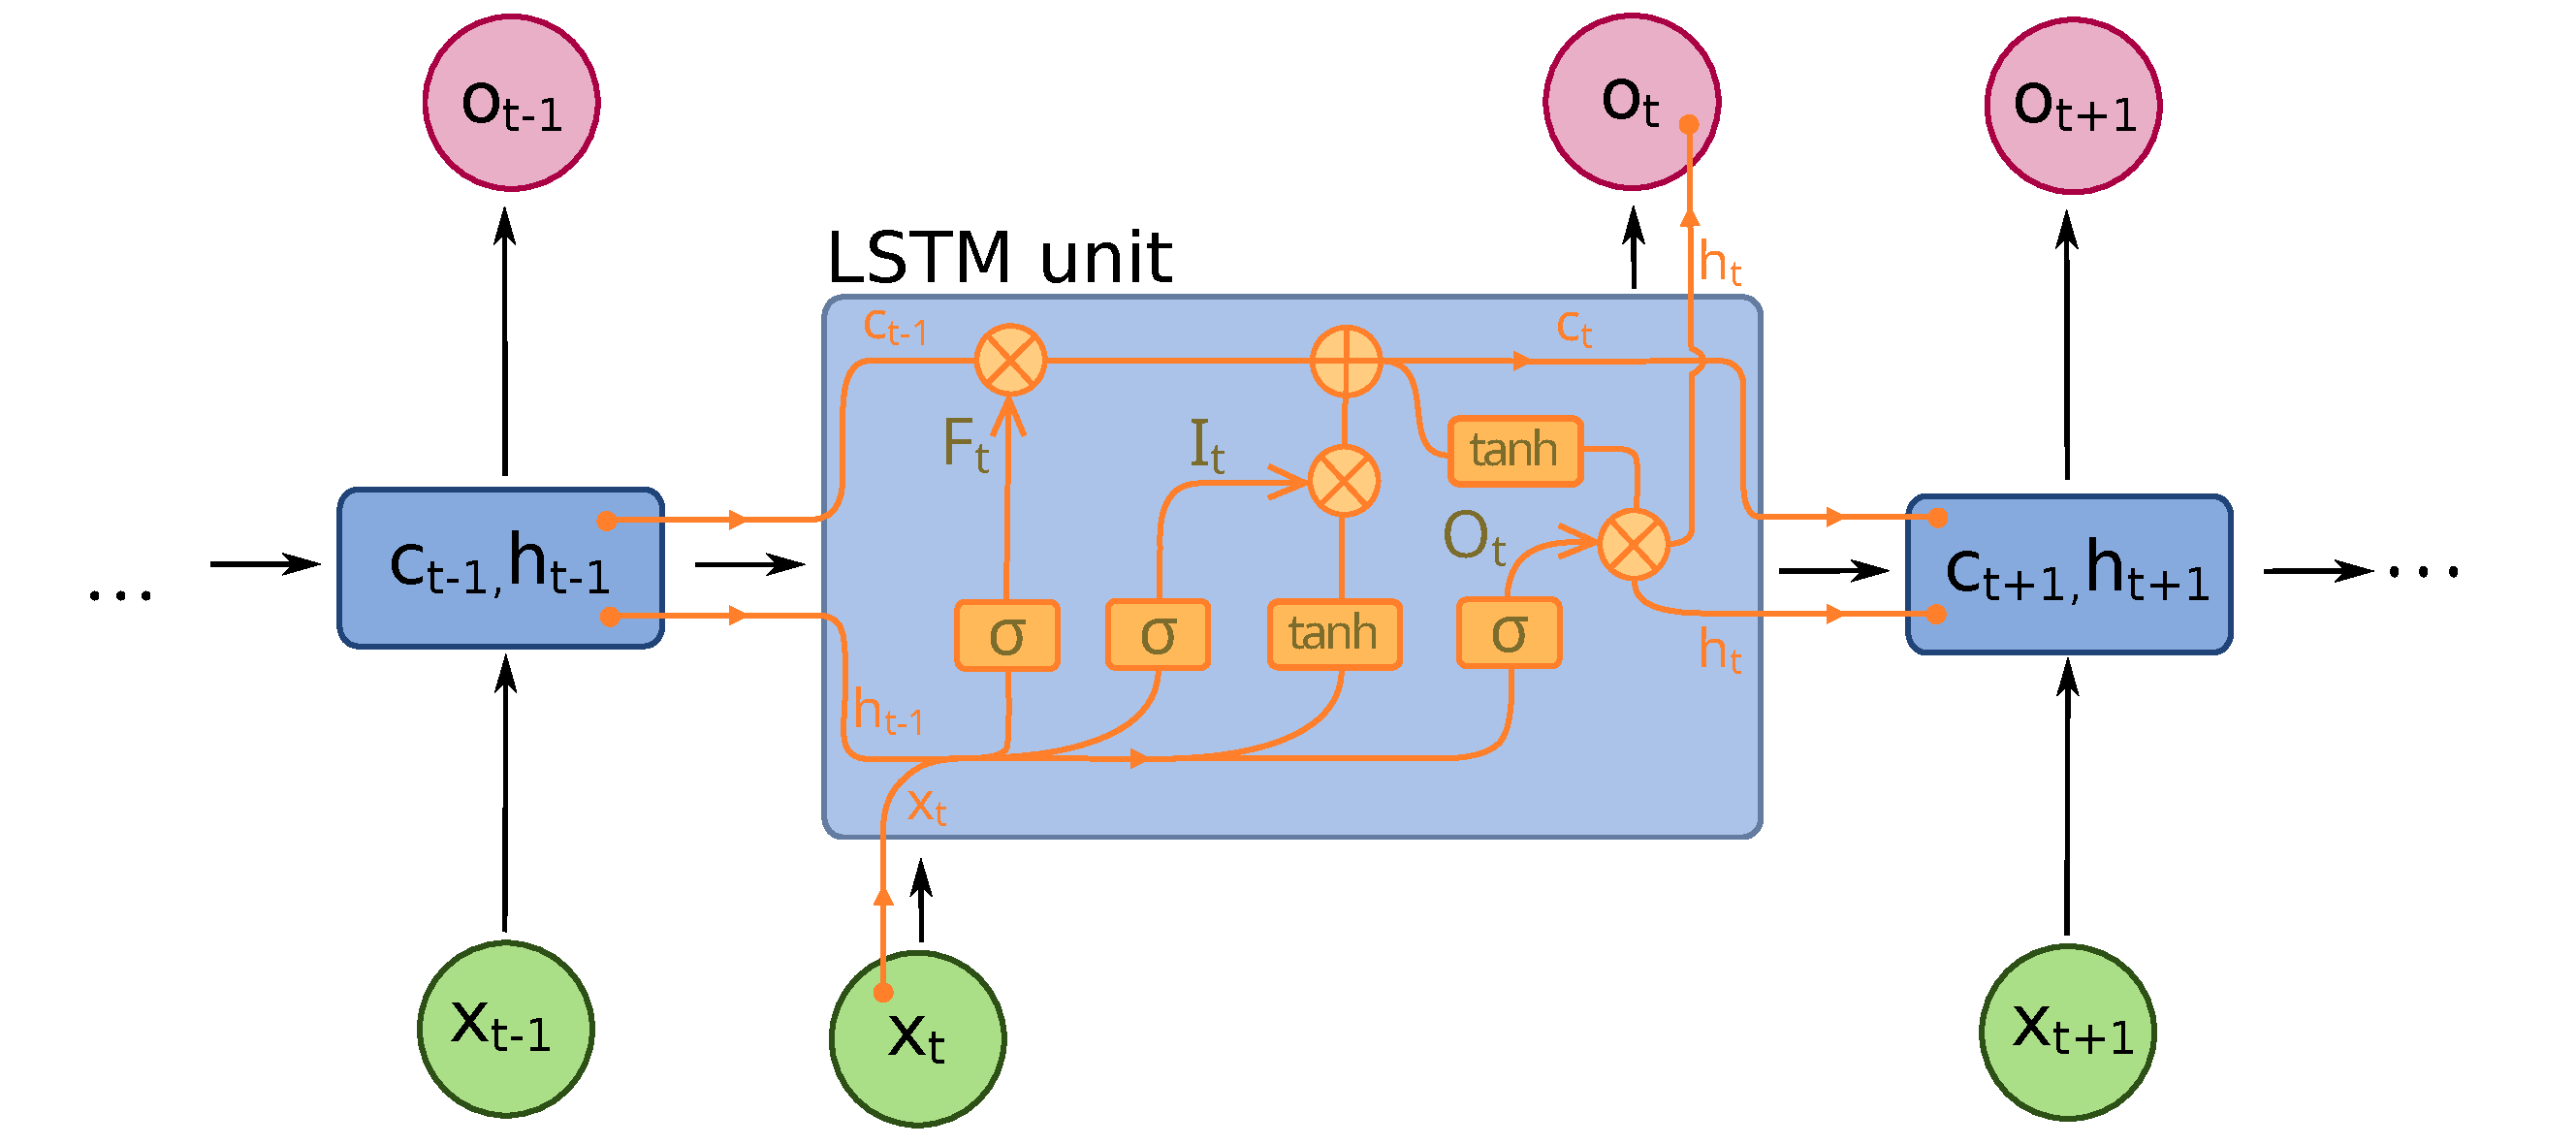
\includegraphics[keepaspectratio]{index_files/mediabag/assets/Long_Short-Term_Memory.pdf}}

\begin{itemize}
\tightlist
\item
  2000-\textgreater2019 : Emergence of Long Short Term Memory models

  \begin{itemize}
  \item
    speech recognition
  \item
    LSTM behind ``Google Translate'', ``Alexa'', \ldots{}
  \end{itemize}
\end{itemize}
\end{frame}

\begin{frame}{The Rise of \emph{transformers}}
\phantomsection\label{the-rise-of-transformers}
A special kind of \textbf{encoder/decoder} architecture.

\begin{columns}[T]
\begin{column}{0.48\linewidth}
Most successful models since 2017

\begin{enumerate}
\tightlist
\item
  Position Encodings

  \begin{itemize}
  \tightlist
  \item
    model is not sequential anymore
  \item
    tries to learn sequence
  \end{itemize}
\item
  \textbf{Attention}

  \begin{itemize}
  \tightlist
  \item
    \href{https://arxiv.org/abs/1706.03762}{attention is all you need}
  \end{itemize}
\item
  Self-Attention
\end{enumerate}
\end{column}

\begin{column}{0.48\linewidth}
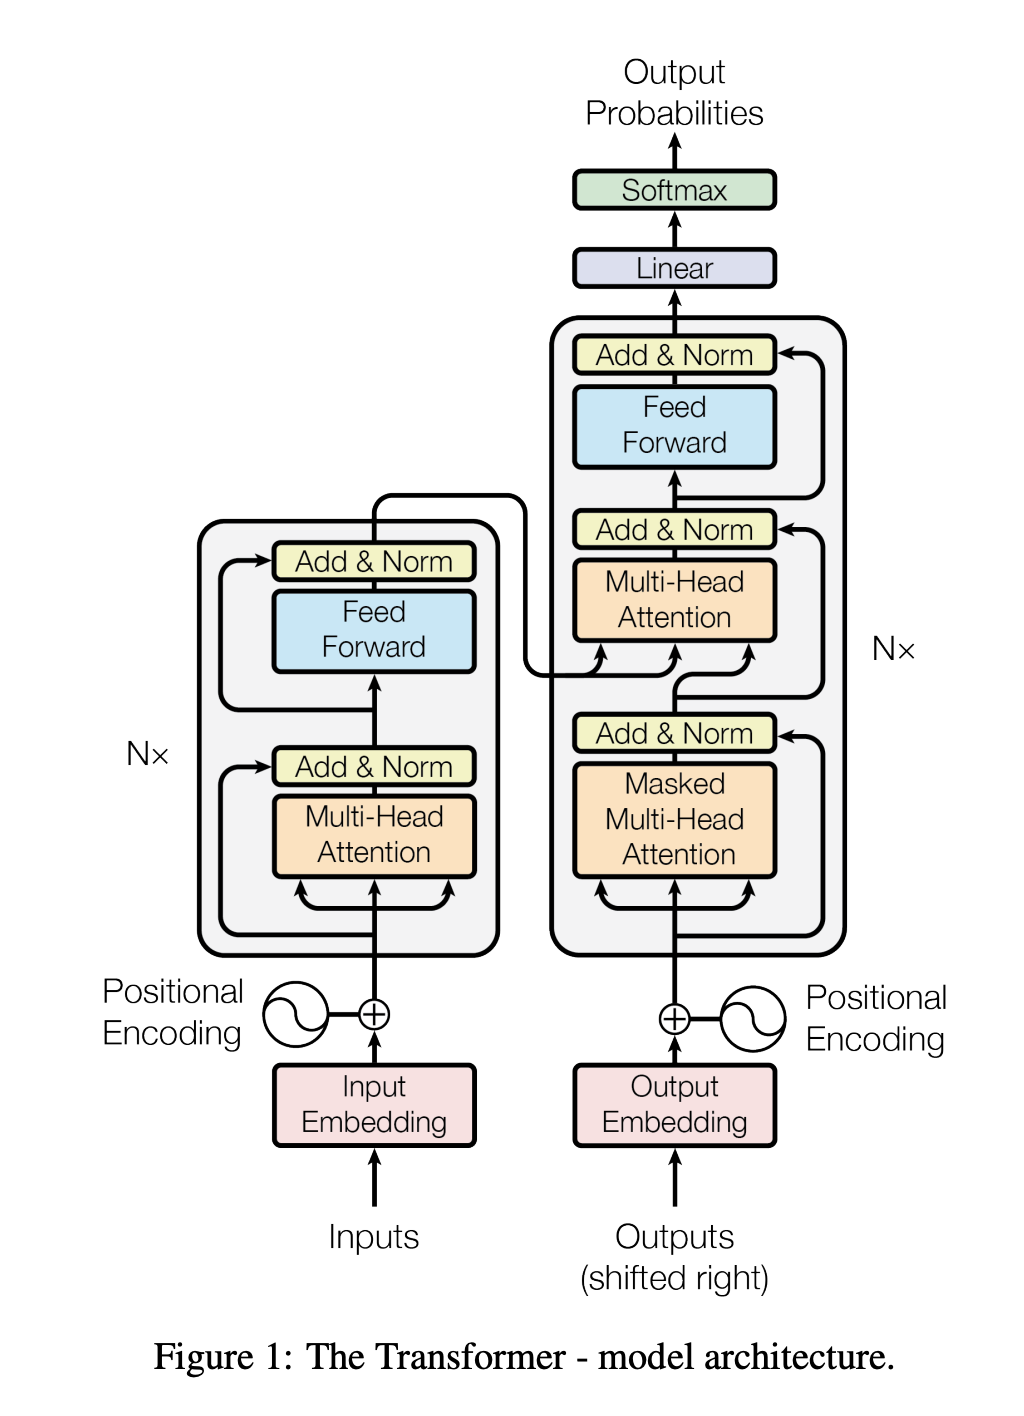
\includegraphics[width=0.6\linewidth,height=\textheight,keepaspectratio]{assets/transformers.png}
\end{column}
\end{columns}

Explanations
\href{https://towardsdatascience.com/transformers-141e32e69591}{here} or
\href{https://blogs.nvidia.com/blog/2022/03/25/what-is-a-transformer-model/}{here}
\end{frame}

\begin{frame}{Encoders / Decoders (1/2)}
\phantomsection\label{encoders-decoders-12}
Take some data \((x_n)\in R^x\).

Consider two functions:

\begin{itemize}
\tightlist
\item
  an \emph{encoder} \[\varphi^E(x; \theta^E) = h \in \mathbb{R^h}\]
\item
  a \emph{decoder}: \[\varphi^D(h; \theta^D) = x' \in \mathbb{R^x}\]
\end{itemize}

What could possibly the value of training the coefficients with:

\[\min_{\theta^E, \theta^D}  \left( \varphi^D( \varphi^E(x_n; \theta^E), \theta^D) - x_n\right)^2\]?

i.e.~train the nets \(\varphi^D\) and \(\varphi^E\) to predict the
``data from the data''? (it is called \textbf{autoencoding})
\end{frame}

\begin{frame}{Encoders / Decoders (2/2)}
\phantomsection\label{encoders-decoders-22}
The relation \(\varphi^D( \varphi^E(x_n; \theta^E), \theta^D) ~ x_n\)
can be rewritten as

\[x_n \xrightarrow{\varphi^E(; \theta^E)} h \xrightarrow{\varphi^D(; \theta^D)} x_n \]

When that relation is (mostly) satisfied and
\(\mathbb{R}^h << \mathbb{R}^x\), \(h\) can be viewed as a lower
dimension representation of \(x\). It encodes the information as a lower
dimension vector \(h\) and is called \textbf{learned embeddings}.

\begin{itemize}
\tightlist
\item
  instead of
  \(\underbrace{x_n}_{\text{prompt}} \rightarrow \underbrace{y_n}_{\text{text completion}}\)
\item
  one can learn
  \(\underbrace{h_n}_{\text{prompt (low dim)}} \xrightarrow{\varphi^C( ; \theta^C)} \underbrace{h_n^c}_{\text{text completion (low dim)}}\)

  \begin{itemize}
  \tightlist
  \item
    it is easier to learn
  \end{itemize}
\item
  and perform the original task as
  \[\underbrace{x_n}_{\text{prompt}} \xrightarrow{\varphi^E}  h_n \xrightarrow{\varphi^C} h_n^C \xrightarrow{\varphi^D} \underbrace{y_n}_{\text{text completion}}\]
\end{itemize}

This very powerful approach can be applied to combine encoders/decoders
from different contexts (ex \href{https://openai.com/dall-e-2}{Dall-E})
\end{frame}

\begin{frame}{Attention}
\phantomsection\label{attention}
Main flaw with the recursive approach:

\begin{itemize}
\tightlist
\item
  the context made to predict new words/embeddings puts a lower weight
  on further words/embeddings
\item
  this is related to the so-called vanishing gradient problem
\end{itemize}

\pause

\begin{columns}[T]
\begin{column}{0.48\linewidth}
With the attention mechanism, each predicted word/embedding is
determined by all preceding words/embeddings, with different weights
that are endogenous.
\end{column}

\begin{column}{0.48\linewidth}
\begin{figure}[H]

{\centering \includegraphics[width=0.5\linewidth,height=\textheight,keepaspectratio]{assets/attention.webp}

}

\caption{Attention}

\end{figure}%
\end{column}
\end{columns}

\pause
\end{frame}

\begin{frame}{Quick summary}
\phantomsection\label{quick-summary}
\begin{itemize}
\tightlist
\item
  Short History of Language models

  \begin{itemize}
  \tightlist
  \item
    frequency tables
  \item
    monte carlo markov chains
  \item
    deep learning -\textgreater{} recurrent neural networks
  \item
    long-short-term memory (\textgreater2000)
  \item
    transformers (\textgreater2018)

    \begin{itemize}
    \tightlist
    \item
      \href{https://arxiv.org/abs/1706.03762}{attention is all you need}
      . . .
    \end{itemize}
  \end{itemize}
\item
  Since 2010 main breakthrough came through the development of
  deep-learning techniques (software/hardware)
\item
  Recently, \emph{models}/algorithms have improved tremendously
\end{itemize}

\pause

More in the next session\ldots{}

In the meantime, checkout the video from 3blue1brown on
\href{https://www.youtube.com/watch?v=eMlx5fFNoYc}{attention}. It's
brilliant!
\end{frame}




\end{document}
